\chapter{Risultati Sperimentali}
\label{chap:chap5}

Il sistema di raccomandazione fuzzy è stato valutato attraverso tre esperimenti progressivi, ciascuno progettato per esplorare aspetti specifici dell'algoritmo e ottimizzare le performance. La progressione degli esperimenti segue un approccio iterativo: dall'esplorazione iniziale dello spazio dei parametri, all'ottimizzazione focalizzata del Fuzzy C-Means, fino al confronto approfondito con il clustering hard tradizionale.

I risultati ottenuti, oltre a essere riportati nel seguente capitolo, sono osservabili nelle cartelle di output del repository. Nel presente capitolo vengono riportati principalmente i plot di comparison (boxplot, heatmap, violinplot, lineplot nclusters) per ciascuna metrica e configurazione e alcuni plot utili per le run migliori, in quanto più sintetici e utili per il confronto tra algoritmi e parametri. Per un'analisi più approfondita e dettagliata, sono disponibili ulteriori visualizzazioni (ad esempio, fuzzy clusters, membership heatmap, membership histogram, ecc.) all'interno delle cartelle di output del repository.

Gli esperimenti sono stati condotti sul dataset MovieLens 100k, filtrato per includere solo utenti e item con almeno 150 rating, risultando in un dataset di circa 300 utenti e 900 film. Questa scelta garantisce una densità di rating sufficiente per valutare l'efficacia del clustering, pur mantenendo la complessità necessaria per testare le capacità del sistema fuzzy.

\section{Metriche}

\subsection{Metriche di Errore Predittivo}

Le metriche RMSE e MAE valutano l'accuratezza predittiva del modello nel prevedere i rating esatti degli utenti. Queste metriche misurano quanto il modello sia preciso nel predire il rating che un utente darebbe a un film specifico.

\subsubsection{RMSE (Root Mean Square Error)}
La metrica RMSE misura l'errore quadratico medio tra i rating predetti e quelli reali. Un valore più basso indica una migliore capacità predittiva. Il RMSE penalizza maggiormente gli errori grandi, rendendolo utile per identificare predizioni molto inaccurate.

\[
RMSE = \sqrt{ \frac{1}{|T|} \sum_{(u,i) \in T} (r_{ui} - \hat{r}_{ui})^2 }
\]

dove:
\begin{itemize}
    \item $T$ è l’insieme delle coppie utente-item nel test set
    \item $r_{ui}$ è il rating reale dell’utente $u$ sull’item $i$
    \item $\hat{r}_{ui}$ è il rating predetto
\end{itemize}

\subsubsection{MAE (Mean Absolute Error)}
La metrica MAE misura l'errore assoluto medio tra i rating predetti e quelli reali. Il MAE è meno sensibile agli outlier rispetto al RMSE e fornisce una misura più robusta degli errori.

\[
MAE = \frac{1}{|T|} \sum_{(u,i) \in T} \left| r_{ui} - \hat{r}_{ui} \right|
\]

dove le variabili sono definite come per il RMSE.

\subsection{Metriche di Qualità delle Raccomandazioni}

Le metriche Precision, Recall, Accuracy e F1-score valutano la qualità effettiva delle raccomandazioni generate dal sistema. A differenza delle metriche di errore che misurano la precisione predittiva dei rating, queste metriche valutano quanto le raccomandazioni siano utili e pertinenti per l'utente nella pratica.

\subsubsection{Precision}
La metrica Precision misura la frazione di item raccomandati nei top-N che sono effettivamente piaciuti all'utente. Un valore più alto indica che il sistema raccomanda principalmente item che l'utente apprezza.

La metrica Precision si calcola come:

\[
Precision = \frac{|\text{Relevant} \cap \text{Recommended}|}{|\text{Recommended}|}
\]

dove:
\begin{itemize}
    \item \textbf{Recommended} è l’insieme degli item raccomandati
    \item \textbf{Relevant} è l’insieme degli item che l’utente ha valutato positivamente (rating $\geq$ soglia)
\end{itemize}

\subsubsection{Recall}
La metrica Recall misura la frazione di item apprezzati dall'utente che sono stati effettivamente raccomandati nei top-N. Un valore più alto indica che il sistema riesce a catturare la maggior parte delle preferenze dell'utente.

La metrica Recall si calcola come:

\[
Recall = \frac{|\text{Relevant} \cap \text{Recommended}|}{|\text{Relevant}|}
\]

dove:
\begin{itemize}
    \item \textbf{Relevant} è l’insieme degli item che l’utente ha effettivamente apprezzato
    \item \textbf{Recommended} è l’insieme degli item suggeriti dal sistema
\end{itemize}


\subsubsection{Accuracy}
La metrica Accuracy misura la frazione di raccomandazioni corrette nei top-N. Questa metrica fornisce una misura diretta dell'accuratezza delle raccomandazioni generate.

La metrica Accuracy si calcola come:

\[
Accuracy = \frac{TP + TN}{TP + TN + FP + FN}
\]

dove:
\begin{itemize}
    \item $TP$ (True Positive): item rilevanti correttamente raccomandati
    \item $TN$ (True Negative): item irrilevanti correttamente non raccomandati
    \item $FP$ (False Positive): item irrilevanti raccomandati
    \item $FN$ (False Negative): item rilevanti non raccomandati
\end{itemize}


\subsubsection{F1-Score}
La metrica F1-Score calcola la media armonica tra Precision e Recall, fornendo una misura bilanciata che considera sia la qualità che la copertura delle raccomandazioni.


\[
F1 = 2 \cdot \frac{Precision \cdot Recall}{Precision + Recall}
\]

Fornisce un compromesso tra qualità (Precision) e copertura (Recall) delle raccomandazioni.


\begin{table}[H]
  \centering
  \begin{tabular}{|l|c|}
  \hline
  \textbf{Metrica} & \textbf{Formula} \\
  \hline
  Precision & $\displaystyle \frac{TP}{TP + FP}$ \\
  Recall & $\displaystyle \frac{TP}{TP + FN}$ \\
  Accuracy & $\displaystyle \frac{TP + TN}{TP + TN + FP + FN}$ \\
  F1-Score & $\displaystyle 2 \cdot \frac{Precision \cdot Recall}{Precision + Recall}$ \\
  \hline
  \end{tabular}
  \caption{Metriche di valutazione delle raccomandazioni}
\end{table}

\section{Run K-Means}

La prima run eseguita è stata la run K-Means, che ha permesso di capire come un algoritmo di hard clustering si comportasse all'interno dello scenario. Per la seguente run, la configurazione utilizzata è la seguente:

\begin{lstlisting}[language=json, caption=Configurazione Run FCM Deep Dive]
{
    "dataset_name": "ml-100k",
    "normalizations": ["no_normalization", "simple_centering", "minmax_per_user", "zscore_per_user"],
    "min_user_ratings": 100,
    "min_item_ratings": 100,
    "cluster_values": [2, 3, 4, 5],
    "m_values": [2.0],
    "noise_std": 0.05,
    "test_size": 0.2,
    "random_state": 42,
    "seed": 31,
    "max_iter": 3000,
    "error": 1e-06,
    "output_dir": "output",
    "show_plots": false,
    "images_subdir": "images",
    "results_subdir": "results",
    "run_timestamp_format": "run_kmeans",
    "clustering_methods": ["kmeans"],
    "defuzzification_methods": ["maximum"],
    "neighbor_selection_methods": ["pearson"],
    "summary_only": false,
    "top_n": 5,
    "top_n_evaluation": {
        "n_recommendations": 10,
        "rating_threshold": 4.0
    }
} 
\end{lstlisting}

Sono quindi stati testati le 4 differenti normalizzazioni, con 2, 3, 4 e 5 cluster. I parametri di fuzziness e defuzzification, sebbene presenti nel config, non sono realmente utilizzati e quindi fungono solo da placeholder.

\subsection{Train}

\begin{table}[H]
  \centering
  \caption{Top 5 Configurazioni per Train RMSE - Run K-Means}
  \resizebox{\textwidth}{!}{%
  \begin{tabular}{|l|c|c|c|c|c|c|c|c|}
  \hline
  \textbf{Rank} & \textbf{Normalization} & \textbf{Clusters} & \textbf{m} & \textbf{Method} & \textbf{Defuzz} & \textbf{Neighbor} & \textbf{Train RMSE} & \textbf{Elapsed Sec}\\
  \hline
  1 & simple\_centering & 5 & 2.0 & kmeans & maximum & pearson & 0.686378 & 41.557193 \\
  2 & simple\_centering & 4 & 2.0 & kmeans & maximum & pearson & 0.686378 & 28.044528 \\
  3 & simple\_centering & 3 & 2.0 & kmeans & maximum & pearson & 0.686378 & 38.488144 \\
  4 & simple\_centering & 2 & 2.0 & kmeans & maximum & pearson & 0.686378 & 40.785123 \\
  5 & zscore\_per\_user & 2 & 2.0 & kmeans & maximum & pearson & 0.712998 & 43.493679 \\
  \hline
  \end{tabular}%
  }
\end{table}

Si osserva che tutte le configurazioni simple\_centering ottengono lo stesso valore di RMSE (0.686378) indipendentemente dal numero di cluster (2-5), suggerendo che il clustering non sta producendo separazioni significative.

\begin{figure}[H]
  \centering
  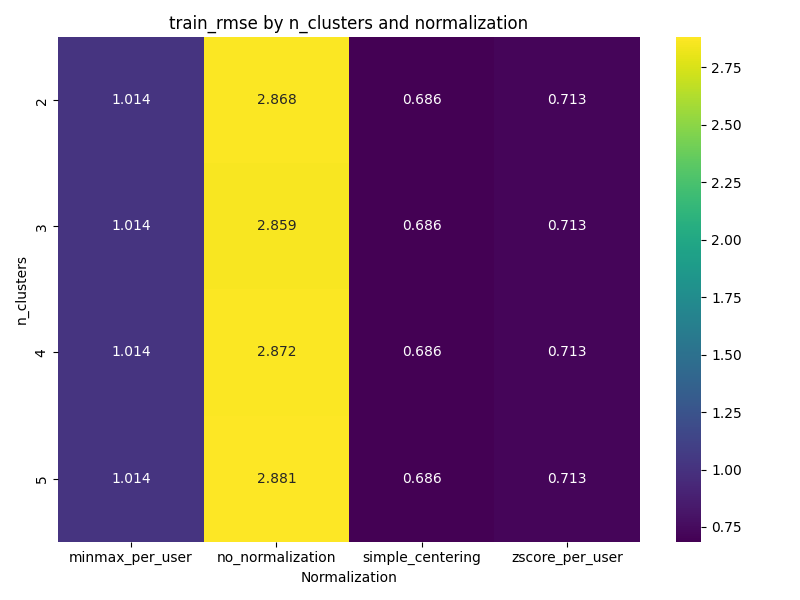
\includegraphics[width=0.8\textwidth]{../output/run_kmeans/images/train/rmse/heatmap_train_rmse.png}
  \caption{Heatmap - Train RMSE - Run K-Means}
  \label{fig:train_rmse_kmeans}
\end{figure}

In figura \ref{fig:train_rmse_kmeans} si può vedere l'heatmap del Train RMSE per le 4 differenti normalizzazioni. Si può confermare come simple\_centering si sia dimostrato il miglior metodo di normalizzazione per K-Means, con il metodo senza normalizzazione che offre le performance peggiori. Eccetto quest'ultima normalizzazione, nelle altre i valori di RMSE rimangono idenici al variare del numero di cluster.

\begin{table}[H]
  \centering
  \caption{Top 5 Configurazioni per Train MAE - Run K-Means}
  \resizebox{\textwidth}{!}{%
  \begin{tabular}{|l|c|c|c|c|c|c|c|c|}
  \hline
  \textbf{Rank} & \textbf{Normalization} & \textbf{Clusters} & \textbf{m} & \textbf{Method} & \textbf{Defuzz} & \textbf{Neighbor} & \textbf{Train MAE} & \textbf{Elapsed Sec}\\
  \hline
  1 & simple\_centering & 5 & 2.0 & kmeans & maximum & pearson & 0.509171 & 41.557193 \\
  2 & simple\_centering & 4 & 2.0 & kmeans & maximum & pearson & 0.509171 & 28.044528 \\
  3 & simple\_centering & 3 & 2.0 & kmeans & maximum & pearson & 0.509171 & 38.488144 \\
  4 & simple\_centering & 2 & 2.0 & kmeans & maximum & pearson & 0.509171 & 40.785123 \\
  5 & zscore\_per\_user & 2 & 2.0 & kmeans & maximum & pearson & 0.537192 & 43.493679 \\
  \hline
  \end{tabular}%
  }
\end{table}

Il pattern è identico al Train RMSE: simple\_centering ottiene lo stesso MAE (0.509171) per tutti i numeri di cluster. Questo conferma la mancanza di separazione significativa tra cluster. Andiamo ad osservarli.

\begin{figure}[H]
  \centering
  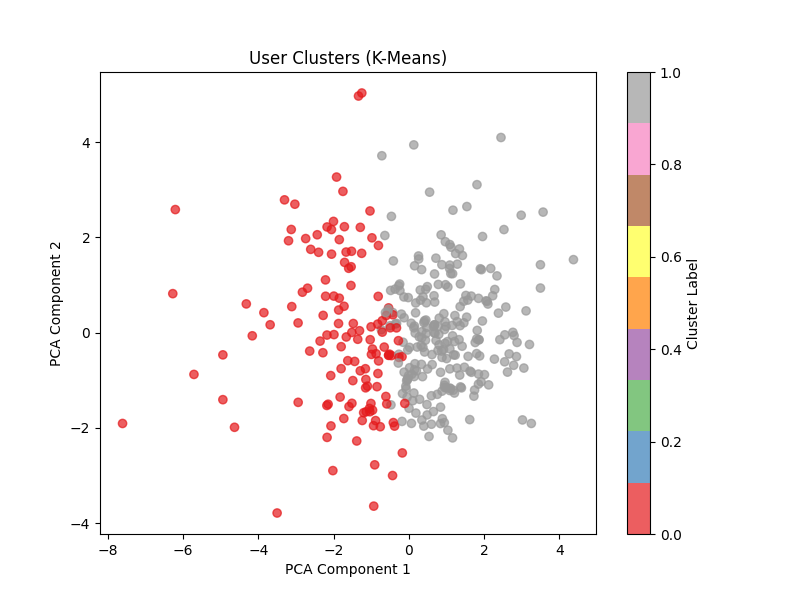
\includegraphics[width=0.5\textwidth]{../output/run_kmeans/images/normalization/simple_centering/hard_clusters/hard_clusters_pca_c2_m2.0_kmeans_maximum_pearson.png}
  \caption{2 Clusters - Run K-Means}
  \label{fig:2_clusters_kmeans}
\end{figure}
\begin{figure}[H]
  \centering
  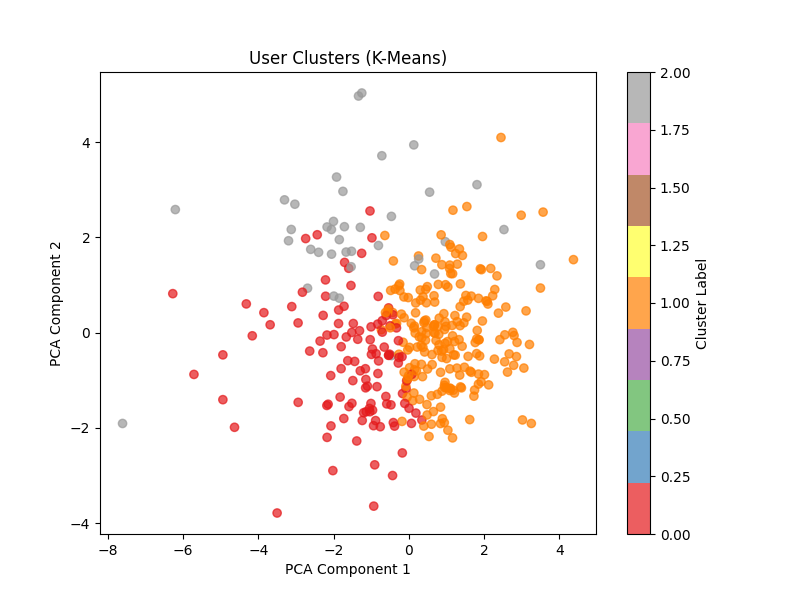
\includegraphics[width=0.5\textwidth]{../output/run_kmeans/images/normalization/simple_centering/hard_clusters/hard_clusters_pca_c3_m2.0_kmeans_maximum_pearson.png}
  \caption{3 Clusters - Run K-Means}
  \label{fig:3_clusters_kmeans}
\end{figure}
\begin{figure}[H]
  \centering
  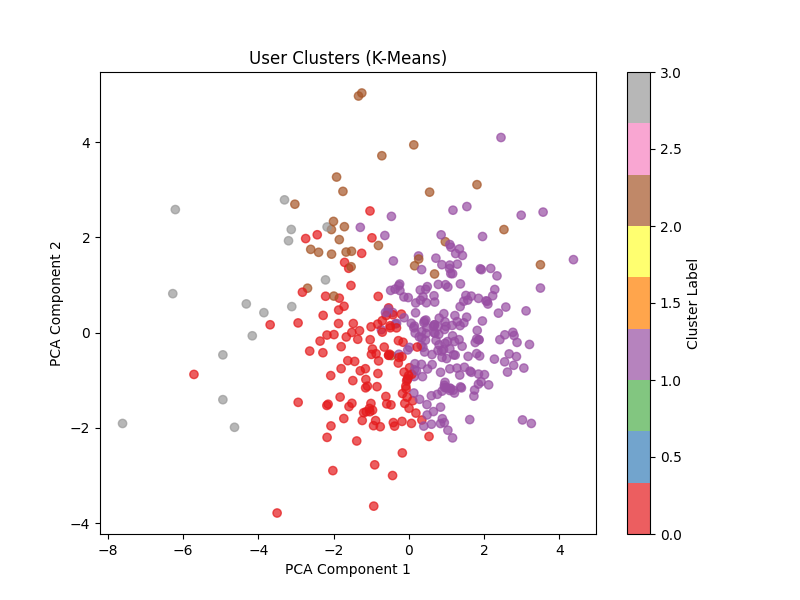
\includegraphics[width=0.5\textwidth]{../output/run_kmeans/images/normalization/simple_centering/hard_clusters/hard_clusters_pca_c4_m2.0_kmeans_maximum_pearson.png}
  \caption{4 Clusters - Run K-Means}
  \label{fig:4_clusters_kmeans}
\end{figure}
\begin{figure}[H]
  \centering
  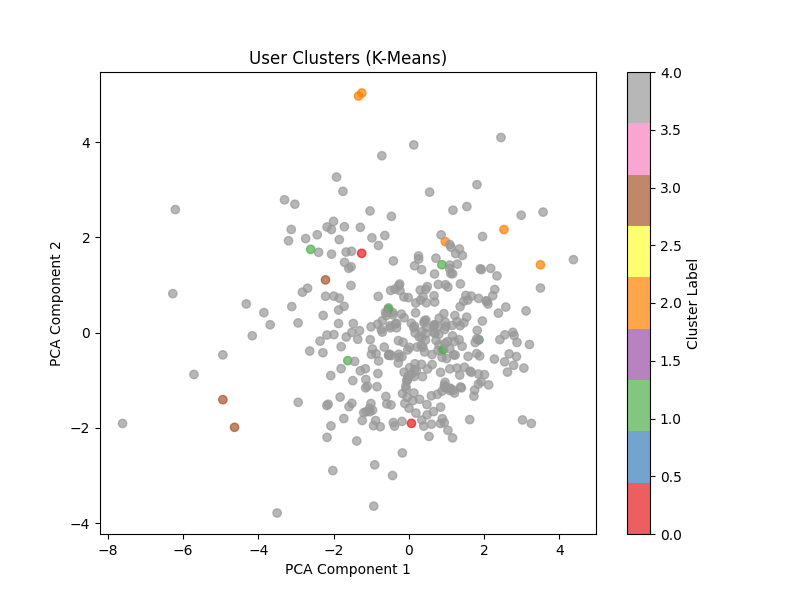
\includegraphics[width=0.5\textwidth]{../output/run_kmeans/images/normalization/simple_centering/hard_clusters/hard_clusters_pca_c5_m2.0_kmeans_maximum_pearson.png}
  \caption{5 Clusters - Run K-Means}
  \label{fig:5_clusters_kmeans}
\end{figure}

Come si può vedere dalle figure \ref{fig:2_clusters_kmeans}, \ref{fig:3_clusters_kmeans}, \ref{fig:4_clusters_kmeans} e \ref{fig:5_clusters_kmeans}, i dati sono molto densi e quindi il clustering non sta producendo separazioni significative, confermando quanto già osservato con le metriche.

\begin{table}[H]
  \centering
  \caption{Top 5 Configurazioni per Train Precision - Run K-Means}
  \resizebox{\textwidth}{!}{%
  \begin{tabular}{|l|c|c|c|c|c|c|c|c|}
  \hline
  \textbf{Rank} & \textbf{Normalization} & \textbf{Clusters} & \textbf{m} & \textbf{Method} & \textbf{Defuzz} & \textbf{Neighbor} & \textbf{Train Precision} & \textbf{Elapsed Sec}\\
  \hline
  1 & no\_normalization & 2 & 2.0 & kmeans & maximum & pearson & 0.588462 & 41.276888 \\
  2 & no\_normalization & 3 & 2.0 & kmeans & maximum & pearson & 0.588187 & 25.853554 \\
  3 & minmax\_per\_user & 3 & 2.0 & kmeans & maximum & pearson & 0.587637 & 21.230663 \\
  4 & minmax\_per\_user & 2 & 2.0 & kmeans & maximum & pearson & 0.587637 & 28.917084 \\
  5 & minmax\_per\_user & 5 & 2.0 & kmeans & maximum & pearson & 0.587637 & 14.610376 \\
  \hline
  \end{tabular}%
  }
\end{table}

Per le metriche di qualità delle raccomandazioni, no\_normalization e minmax\_per\_user dominano, a differenza delle metriche di errore. I valori di precision sono simili (~0.587-0.588) indipendentemente dal numero di cluster.

\begin{figure}[H]
  \centering
  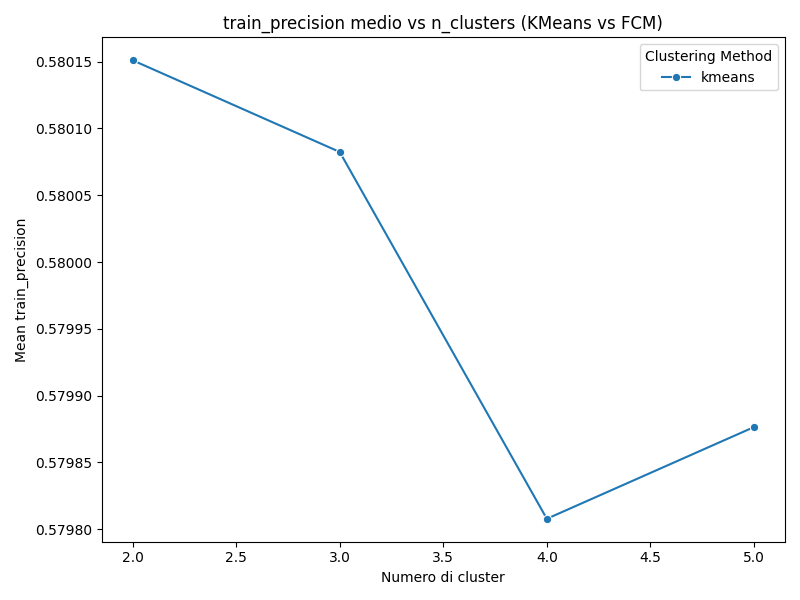
\includegraphics[width=0.8\textwidth]{../output/run_kmeans/images/train/precision/lineplot_nclusters_train_precision.png}
  \caption{Lineplot - Train Precision - Run K-Means}
  \label{fig:train_precision_kmeans}
\end{figure}

In figura \ref{fig:train_precision_kmeans} si può vedere il lineplot del Train Precision all'aumentare del numero di cluster. Si può notare come il valore di precision sia più alto con numero di cluster basso, sebbene con 5 fornisca una risalita rispetto a 4. 

\begin{table}[H]
  \centering
  \caption{Top 5 Configurazioni per Train Recall - Run K-Means}
  \resizebox{\textwidth}{!}{%
  \begin{tabular}{|l|c|c|c|c|c|c|c|c|}
  \hline
  \textbf{Rank} & \textbf{Normalization} & \textbf{Clusters} & \textbf{m} & \textbf{Method} & \textbf{Defuzz} & \textbf{Neighbor} & \textbf{Train Recall} & \textbf{Elapsed Sec}\\
  \hline
  1 & no\_normalization & 3 & 2.0 & kmeans & maximum & pearson & 0.138107 & 25.853554 \\
  2 & no\_normalization & 2 & 2.0 & kmeans & maximum & pearson & 0.138094 & 41.276888 \\
  3 & no\_normalization & 4 & 2.0 & kmeans & maximum & pearson & 0.137644 & 19.790054 \\
  4 & no\_normalization & 5 & 2.0 & kmeans & maximum & pearson & 0.137630 & 18.933092 \\
  5 & minmax\_per\_user & 5 & 2.0 & kmeans & maximum & pearson & 0.137605 & 14.610376 \\
  \hline
  \end{tabular}%
  }
\end{table}

I valori di recall sono molto bassi (~0.137-0.138). no\_normalization domina con valori leggermente decrescenti all'aumentare del numero di cluster, suggerendo un leggero overfitting, così come avveniva in precision.

\begin{table}[H]
  \centering
  \caption{Top 5 Configurazioni per Train Accuracy - Run K-Means}
  \resizebox{\textwidth}{!}{%
  \begin{tabular}{|l|c|c|c|c|c|c|c|c|}
  \hline
  \textbf{Rank} & \textbf{Normalization} & \textbf{Clusters} & \textbf{m} & \textbf{Method} & \textbf{Defuzz} & \textbf{Neighbor} & \textbf{Train Accuracy} & \textbf{Elapsed Sec}\\
  \hline
  1 & no\_normalization & 2 & 2.0 & kmeans & maximum & pearson & 0.588462 & 41.276888 \\
  2 & no\_normalization & 3 & 2.0 & kmeans & maximum & pearson & 0.588187 & 25.853554 \\
  3 & minmax\_per\_user & 3 & 2.0 & kmeans & maximum & pearson & 0.587637 & 21.230663 \\
  4 & minmax\_per\_user & 2 & 2.0 & kmeans & maximum & pearson & 0.587637 & 28.917084 \\
  5 & minmax\_per\_user & 5 & 2.0 & kmeans & maximum & pearson & 0.587637 & 14.610376 \\
  \hline
  \end{tabular}%
  }
\end{table}

I risultati sono identici al Train Precision, confermando che accuracy e precision coincidono.

\begin{figure}[H]
  \centering
  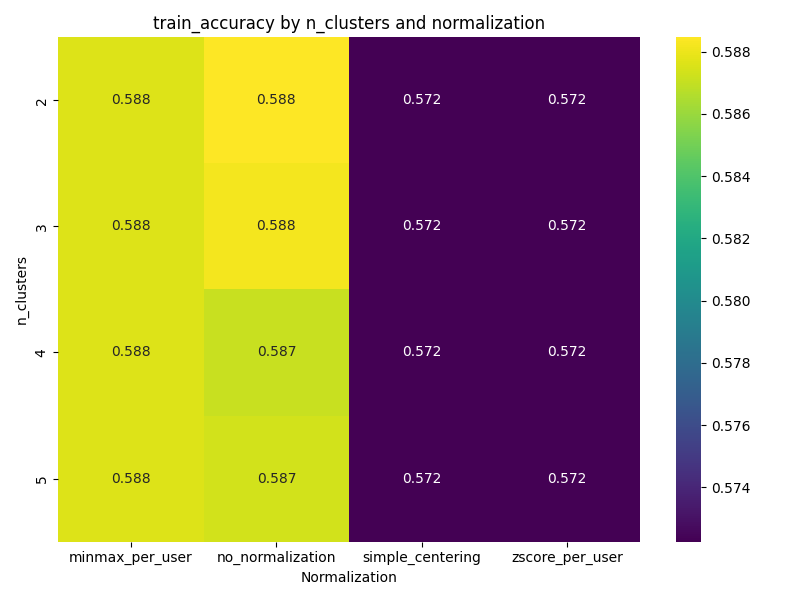
\includegraphics[width=0.8\textwidth]{../output/run_kmeans/images/train/accuracy/heatmap_train_accuracy.png}
  \caption{Heatmap - Train Accuracy - Run K-Means}
  \label{fig:train_accuracy_kmeans}
\end{figure}

In figura \ref{fig:train_accuracy_kmeans} si può osservare un risultato interessante: il clustering senza normalizzazione offre prestazioni simili alle tre tecniche di normalizzazione considerate, suggerendo che, almeno in questo contesto e con questi dati, le caratteristiche intrinseche dei dati sono già ben rappresentate senza la necessità di trasformazioni aggiuntive.

\begin{table}[H]
  \centering
  \caption{Top 5 Configurazioni per Train F1-Score - Run K-Means}
  \resizebox{\textwidth}{!}{%
  \begin{tabular}{|l|c|c|c|c|c|c|c|c|}
  \hline
  \textbf{Rank} & \textbf{Normalization} & \textbf{Clusters} & \textbf{m} & \textbf{Method} & \textbf{Defuzz} & \textbf{Neighbor} & \textbf{Train F1-Score} & \textbf{Elapsed Sec}\\
  \hline
  1 & no\_normalization & 2 & 2.0 & kmeans & maximum & pearson & 0.210876 & 41.276888 \\
  2 & no\_normalization & 3 & 2.0 & kmeans & maximum & pearson & 0.210854 & 25.853554 \\
  3 & minmax\_per\_user & 3 & 2.0 & kmeans & maximum & pearson & 0.210282 & 21.230663 \\
  4 & minmax\_per\_user & 2 & 2.0 & kmeans & maximum & pearson & 0.210282 & 28.917084 \\
  5 & minmax\_per\_user & 5 & 2.0 & kmeans & maximum & pearson & 0.210282 & 14.610376 \\
  \hline
  \end{tabular}%
  }
\end{table}

Gli F1-score sono bassi (~0.21) a causa dei valori di recall molto bassi. no\_normalization ottiene i migliori risultati, con valori leggermente decrescenti all'aumentare del numero di cluster.

\subsection{Test}

\begin{table}[H]
  \centering
  \caption{Top 5 Configurazioni per Test RMSE - Run K-Means}
  \resizebox{\textwidth}{!}{%
  \begin{tabular}{|l|c|c|c|c|c|c|c|c|}
  \hline
  \textbf{Rank} & \textbf{Normalization} & \textbf{Clusters} & \textbf{m} & \textbf{Method} & \textbf{Defuzz} & \textbf{Neighbor} & \textbf{Test RMSE} & \textbf{Elapsed Sec}\\
  \hline
  1 & simple\_centering & 2 & 2.0 & kmeans & maximum & pearson & 0.681716 & 40.785123 \\
  2 & simple\_centering & 3 & 2.0 & kmeans & maximum & pearson & 0.681716 & 38.488144 \\
  3 & simple\_centering & 4 & 2.0 & kmeans & maximum & pearson & 0.681716 & 28.044528 \\
  4 & simple\_centering & 5 & 2.0 & kmeans & maximum & pearson & 0.681716 & 41.557193 \\
  5 & minmax\_per\_user & 5 & 2.0 & kmeans & maximum & pearson & 0.699511 & 14.610376 \\
  \hline
  \end{tabular}%
  }
\end{table}

Anche nel test, simple\_centering ottiene lo stesso RMSE (0.681716) per tutti i numeri di cluster. Il Test RMSE è leggermente migliore del Train RMSE, indicando una buona generalizzazione.

\begin{figure}[H]
  \centering
  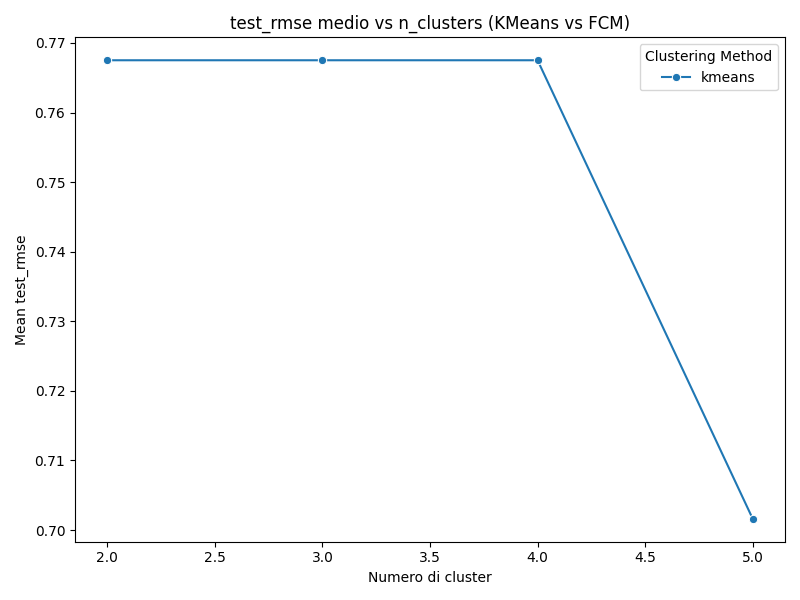
\includegraphics[width=0.8\textwidth]{../output/run_kmeans/images/test/rmse/lineplot_nclusters_test_rmse.png}
  \caption{Heatmap - Test RMSE - Run K-Means}
  \label{fig:test_rmse_kmeans}
\end{figure}

Dalla figura \ref{fig:test_rmse_kmeans} si può osservare che, in realtà, con 5 cluster, il Test RMSE peggiora notevolmente rispetto agli altri valori.


\begin{table}[H]
  \centering
  \caption{Top 5 Configurazioni per Test MAE - Run K-Means}
  \resizebox{\textwidth}{!}{%
  \begin{tabular}{|l|c|c|c|c|c|c|c|c|}
  \hline
  \textbf{Rank} & \textbf{Normalization} & \textbf{Clusters} & \textbf{m} & \textbf{Method} & \textbf{Defuzz} & \textbf{Neighbor} & \textbf{Test MAE} & \textbf{Elapsed Sec}\\
  \hline
  1 & zscore\_per\_user & 5 & 2.0 & kmeans & maximum & pearson & 0.540973 & 38.939321 \\
  2 & zscore\_per\_user & 4 & 2.0 & kmeans & maximum & pearson & 0.540973 & 45.033325 \\
  3 & zscore\_per\_user & 3 & 2.0 & kmeans & maximum & pearson & 0.540973 & 37.246547 \\
  4 & zscore\_per\_user & 2 & 2.0 & kmeans & maximum & pearson & 0.540973 & 43.493679 \\
  5 & simple\_centering & 2 & 2.0 & kmeans & maximum & pearson & 0.547638 & 40.785123 \\
  \hline
  \end{tabular}%
  }
\end{table}

A differenza delle altre metriche, zscore\_per\_user domina il Test MAE con lo stesso valore (0.540973) per tutti i numeri di cluster. Questo suggerisce una diversa sensibilità della metrica MAE alla normalizzazione.

\begin{figure}[H]
  \centering
  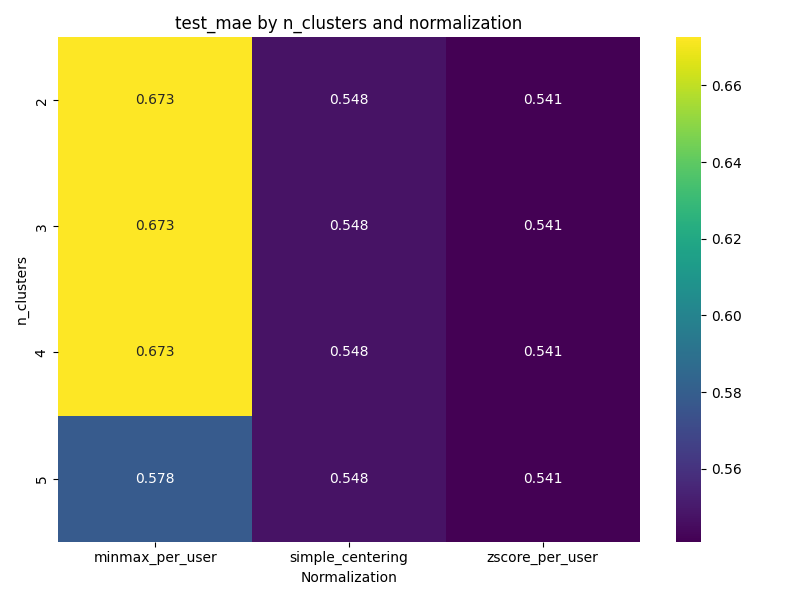
\includegraphics[width=0.8\textwidth]{../output/run_kmeans/images/test/mae/heatmap_test_mae.png}
  \caption{Heatmap - Test MAE - Run K-Means}
  \label{fig:test_mae_kmeans}
\end{figure}

In figura \ref{fig:test_mae_kmeans} possiamo confermare quanto emerso dalla tabella: zscore\_per\_user offre prestazioni migliori rispetto alle altre normalizzazioni.

\begin{table}[H]
  \centering
  \caption{Top 5 Configurazioni per Test Precision - Run K-Means}
  \resizebox{\textwidth}{!}{%
  \begin{tabular}{|l|c|c|c|c|c|c|c|c|}
  \hline
  \textbf{Rank} & \textbf{Normalization} & \textbf{Clusters} & \textbf{m} & \textbf{Method} & \textbf{Defuzz} & \textbf{Neighbor} & \textbf{Test Precision} & \textbf{Elapsed Sec}\\
  \hline
  1 & simple\_centering & 5 & 2.0 & kmeans & maximum & pearson & 0.605029 & 41.557193 \\
  2 & simple\_centering & 4 & 2.0 & kmeans & maximum & pearson & 0.605029 & 28.044528 \\
  3 & simple\_centering & 3 & 2.0 & kmeans & maximum & pearson & 0.605029 & 38.488144 \\
  4 & simple\_centering & 2 & 2.0 & kmeans & maximum & pearson & 0.605029 & 40.785123 \\
  5 & zscore\_per\_user & 2 & 2.0 & kmeans & maximum & pearson & 0.605029 & 43.493679 \\
  \hline
  \end{tabular}%
  }
\end{table}

A differenza del train, simple\_centering domina il Test Precision con lo stesso valore (0.605029) per tutti i numeri di cluster. Questo valore è identico al miglior risultato FCM, suggerendo performance simili.

\begin{table}[H]
  \centering
  \caption{Top 5 Configurazioni per Test Recall - Run K-Means}
  \resizebox{\textwidth}{!}{%
  \begin{tabular}{|l|c|c|c|c|c|c|c|c|}
  \hline
  \textbf{Rank} & \textbf{Normalization} & \textbf{Clusters} & \textbf{m} & \textbf{Method} & \textbf{Defuzz} & \textbf{Neighbor} & \textbf{Test Recall} & \textbf{Elapsed Sec}\\
  \hline
  1 & simple\_centering & 5 & 2.0 & kmeans & maximum & pearson & 0.511998 & 41.557193 \\
  2 & simple\_centering & 4 & 2.0 & kmeans & maximum & pearson & 0.511998 & 28.044528 \\
  3 & simple\_centering & 3 & 2.0 & kmeans & maximum & pearson & 0.511998 & 38.488144 \\
  4 & simple\_centering & 2 & 2.0 & kmeans & maximum & pearson & 0.511998 & 40.785123 \\
  5 & zscore\_per\_user & 2 & 2.0 & kmeans & maximum & pearson & 0.511835 & 43.493679 \\
  \hline
  \end{tabular}%
  }
\end{table}

Il pattern è identico al Test Precision. I valori di recall (~0.51) sono molto più alti rispetto al train (~0.14), identici a FCM. Questo suggerisce una migliore capacità di generalizzazione per entrambi gli algoritmi.

\begin{table}[H]
  \centering
  \caption{Top 5 Configurazioni per Test Accuracy - Run K-Means}
  \resizebox{\textwidth}{!}{%
  \begin{tabular}{|l|c|c|c|c|c|c|c|c|}
  \hline
  \textbf{Rank} & \textbf{Normalization} & \textbf{Clusters} & \textbf{m} & \textbf{Method} & \textbf{Defuzz} & \textbf{Neighbor} & \textbf{Test Accuracy} & \textbf{Elapsed Sec}\\
  \hline
  1 & simple\_centering & 5 & 2.0 & kmeans & maximum & pearson & 0.605029 & 41.557193 \\
  2 & simple\_centering & 4 & 2.0 & kmeans & maximum & pearson & 0.605029 & 28.044528 \\
  3 & simple\_centering & 3 & 2.0 & kmeans & maximum & pearson & 0.605029 & 38.488144 \\
  4 & simple\_centering & 2 & 2.0 & kmeans & maximum & pearson & 0.605029 & 40.785123 \\
  5 & zscore\_per\_user & 2 & 2.0 & kmeans & maximum & pearson & 0.605029 & 43.493679 \\
  \hline
  \end{tabular}%
  }
\end{table}

I risultati sono identici al Test Precision, confermando che accuracy e precision coincidono anche per K-Means nella fase di test. Questo pattern è consistente con FCM.

\begin{table}[H]
  \centering
  \caption{Top 5 Configurazioni per Test F1-Score - Run K-Means}
  \resizebox{\textwidth}{!}{%
  \begin{tabular}{|l|c|c|c|c|c|c|c|c|}
  \hline
  \textbf{Rank} & \textbf{Normalization} & \textbf{Clusters} & \textbf{m} & \textbf{Method} & \textbf{Defuzz} & \textbf{Neighbor} & \textbf{Test F1-Score} & \textbf{Elapsed Sec}\\
  \hline
  1 & simple\_centering & 5 & 2.0 & kmeans & maximum & pearson & 0.524162 & 41.557193 \\
  2 & simple\_centering & 4 & 2.0 & kmeans & maximum & pearson & 0.524162 & 28.044528 \\
  3 & simple\_centering & 3 & 2.0 & kmeans & maximum & pearson & 0.524162 & 38.488144 \\
  4 & simple\_centering & 2 & 2.0 & kmeans & maximum & pearson & 0.524162 & 40.785123 \\
  5 & zscore\_per\_user & 2 & 2.0 & kmeans & maximum & pearson & 0.524015 & 43.493679 \\
  \hline
  \end{tabular}%
  }
\end{table}

Gli F1-score (~0.52) sono significativamente più alti rispetto al train (~0.21) grazie ai valori di recall più elevati, identici a FCM. Il pattern di normalizzazione e cluster è identico alle altre metriche di test.

\subsection{Conclusioni K-Means}

I risultati della run K-Means rivelano pattern interessanti.

Per quanto riguarda le metriche RMSE e MAE, simple\_centering emerge come la normalizzazione dominante sia in fase di train che di test. I valori di RMSE (~0.68-0.69) e MAE (~0.51-0.55) indicano che il sistema commette errori medi di circa 0.7 stelle su una scala da 1 a 5 nel predire i rating degli utenti. Questo significa che se un utente ha dato 4 stelle a un film, il sistema potrebbe prevedere 3.3 o 4.7 stelle. Nel contesto pratico, questo livello di errore è accettabile per un sistema di raccomandazione, considerando che la scala di rating è soggettiva e che differenze di 0.5-1 stella sono spesso considerate normali tra utenti diversi.

La mancanza di variazione nei valori di errore al variare del numero di cluster (2-5) suggerisce che il clustering non sta producendo separazioni significative tra i profili utente. Questo fenomeno può essere interpretato positivamente: indica che gli utenti del dataset MovieLens 100k, dopo il filtraggio per densità, mostrano preferenze cinematografiche relativamente omogenee. In pratica, questo significa che la maggior parte degli utenti attivi (con almeno 150 rating) tende ad apprezzare film simili, rendendo difficile identificare cluster distinti di gusti cinematografici.

Le metriche di qualità rivelano una dicotomia interessante tra fase di train e test. In training, no\_normalization e minmax\_per\_user dominano con valori di precision e accuracy intorno al 58.8\%. Questo significa che il 58.8\% dei film raccomandati dal sistema sono effettivamente apprezzati dall'utente (rating $\geq$ 4.0). Tuttavia, i valori di recall molto bassi (~13.8\%) indicano che il sistema riesce a catturare solo una piccola frazione degli item che l'utente apprezza.

In fase di test, si osserva un miglioramento significativo: simple\_centering domina con precision/accuracy del 60.5\% e recall del 51.2\%. Questo miglioramento suggerisce che il sistema generalizza bene su nuovi dati, riuscendo a catturare una porzione maggiore delle preferenze dell'utente. Il fatto che il recall raddoppi quasi (da 13.8\% a 51.2\%) indica una migliore capacità di scoprire film che l'utente potrebbe apprezzare ma non ha ancora valutato.

\section{Run FCM}

Una volta eseguita la run con K-Means e analizzati i risultati, si è deciso di eseguire una run con FCM per capire se un algoritmo fuzzy può migliorare le prestazioni permettendo di catturare la sfumatura delle preferenze cinematografiche degli utenti.

\subsection{Train}

\begin{table}[H]
  \centering
  \caption{Top 5 Configurazioni per Train RMSE - Run FCM}
  \resizebox{\textwidth}{!}{%
  \begin{tabular}{|l|c|c|c|c|c|c|c|c|c|c|}
  \hline
  \textbf{Rank} & \textbf{Normalization} & \textbf{Clusters} & \textbf{m} & \textbf{Method} & \textbf{Defuzz} & \textbf{Neighbor} & \textbf{Train RMSE} & \textbf{Avg Max Membership} & \textbf{Avg Entropy} & \textbf{Elapsed Sec}\\
  \hline
  1 & simple\_centering & 2 & 1.2 & fcm & maximum & pearson & 0.685134 & 0.5 & 0.693147 & 39.334954 \\
  2 & simple\_centering & 2 & 1.2 & fcm & cog & pearson & 0.685134 & 0.5 & 0.693147 & 39.532738 \\
  3 & simple\_centering & 2 & 1.5 & fcm & maximum & pearson & 0.685134 & 0.5 & 0.693147 & 39.051460 \\
  4 & simple\_centering & 2 & 1.5 & fcm & cog & pearson & 0.685134 & 0.5 & 0.693147 & 39.617368 \\
  5 & simple\_centering & 2 & 1.8 & fcm & maximum & pearson & 0.685134 & 0.5 & 0.693147 & 39.740233 \\
  \hline
  \end{tabular}%
  }
\end{table}

Si osserva che tutte le configurazioni ottimali utilizzano simple\_centering con 2 cluster, indipendentemente dal valore di fuzziness (m) e dal metodo di defuzzificazione. I valori di Avg Max Membership (0.5) e Avg Entropy (0.693) sono identici per tutte le configurazioni, suggerendo una distribuzione uniforme delle membership.

\begin{figure}[H]
  \centering
  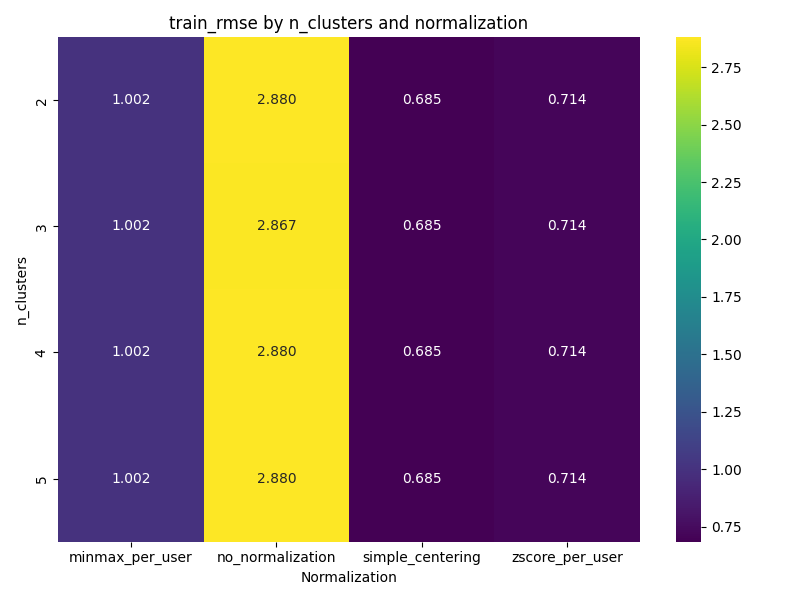
\includegraphics[width=0.8\textwidth]{../output/run_fcm/images/train/rmse/heatmap_train_rmse.png}
  \caption{Heatmap - Train RMSE - Run FCM}
  \label{fig:train_rmse_fcm}
\end{figure}

In figura \ref{fig:train_rmse_fcm} si può confermare come simple\_centering offre prestazioni migliori rispetto alle altre configurazioni.

\begin{table}[H]
  \centering
  \caption{Top 5 Configurazioni per Train MAE - Run FCM}
  \resizebox{\textwidth}{!}{%
  \begin{tabular}{|l|c|c|c|c|c|c|c|c|c|c|}
  \hline
  \textbf{Rank} & \textbf{Normalization} & \textbf{Clusters} & \textbf{m} & \textbf{Method} & \textbf{Defuzz} & \textbf{Neighbor} & \textbf{Train MAE} & \textbf{Avg Max Membership} & \textbf{Avg Entropy} & \textbf{Elapsed Sec}\\
  \hline
  1 & simple\_centering & 2 & 1.2 & fcm & maximum & pearson & 0.510734 & 0.5 & 0.693147 & 39.334954 \\
  2 & simple\_centering & 2 & 1.2 & fcm & cog & pearson & 0.510734 & 0.5 & 0.693147 & 39.532738 \\
  3 & simple\_centering & 2 & 1.5 & fcm & maximum & pearson & 0.510734 & 0.5 & 0.693147 & 39.051460 \\
  4 & simple\_centering & 2 & 1.5 & fcm & cog & pearson & 0.510734 & 0.5 & 0.693147 & 39.617368 \\
  5 & simple\_centering & 2 & 1.8 & fcm & maximum & pearson & 0.510734 & 0.5 & 0.693147 & 39.740233 \\
  \hline
  \end{tabular}%
  }
\end{table}

Il pattern è identico al Train RMSE: simple\_centering con 2 cluster domina, con valori identici di MAE, Avg Max Membership e Avg Entropy per tutte le configurazioni. Questo suggerisce che il numero di cluster ha un impatto maggiore dei parametri di fuzziness.

\begin{table}[H]
  \centering
  \caption{Top 5 Configurazioni per Train Precision - Run FCM}
  \resizebox{\textwidth}{!}{%
  \begin{tabular}{|l|c|c|c|c|c|c|c|c|c|c|}
  \hline
  \textbf{Rank} & \textbf{Normalization} & \textbf{Clusters} & \textbf{m} & \textbf{Method} & \textbf{Defuzz} & \textbf{Neighbor} & \textbf{Train Precision} & \textbf{Avg Max Membership} & \textbf{Avg Entropy} & \textbf{Elapsed Sec}\\
  \hline
  1 & no\_normalization & 3 & 1.2 & fcm & cog & pearson & 0.589011 & 0.446683 & 1.019679 & 43.236223 \\
  2 & no\_normalization & 2 & 1.2 & fcm & maximum & pearson & 0.588187 & 0.621032 & 0.645280 & 40.750197 \\
  3 & no\_normalization & 2 & 1.5 & fcm & maximum & pearson & 0.588187 & 0.5 & 0.693147 & 42.361609 \\
  4 & no\_normalization & 2 & 1.2 & fcm & cog & pearson & 0.588187 & 0.621032 & 0.645280 & 41.118601 \\
  5 & no\_normalization & 2 & 1.8 & fcm & maximum & pearson & 0.588187 & 0.5 & 0.693147 & 41.554277 \\
  \hline
  \end{tabular}%
  }
\end{table}

Per le metriche di qualità delle raccomandazioni, no\_normalization domina le classifiche. Si nota una correlazione tra Avg Max Membership e Avg Entropy: valori più alti di membership corrispondono a entropia più bassa, indicando cluster più definiti. I valori, inoltre, non sono più esattamente 0.5 e 0.693 come in K-Means, ma sono leggermente diversi, indicando che il clustering fuzzy produce cluster più sfumati.

\begin{figure}[H]
  \centering
  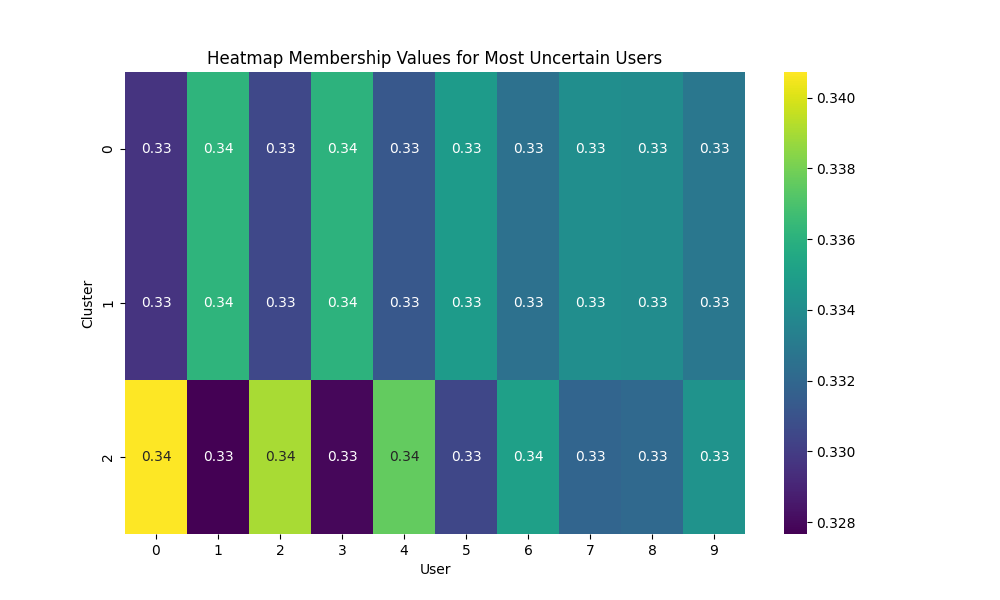
\includegraphics[width=0.8\textwidth]{../output/run_fcm/images/normalization/no_normalization/membership_heatmap/membership_heatmap_c3_m1.2_fcm_cog_pearson.png}
  \caption{Heatmap - Train Precision - Run FCM}
  \label{fig:train_precision_fcm}
\end{figure}

In figura \ref{fig:train_precision_fcm} si può confermare questa leggera sfumatura dei cluster.

\begin{table}[H]
  \centering
  \caption{Top 5 Configurazioni per Train Recall - Run FCM}
  \resizebox{\textwidth}{!}{%
  \begin{tabular}{|l|c|c|c|c|c|c|c|c|c|c|}
  \hline
  \textbf{Rank} & \textbf{Normalization} & \textbf{Clusters} & \textbf{m} & \textbf{Method} & \textbf{Defuzz} & \textbf{Neighbor} & \textbf{Train Recall} & \textbf{Avg Max Membership} & \textbf{Avg Entropy} & \textbf{Elapsed Sec}\\
  \hline
  1 & no\_normalization & 3 & 1.2 & fcm & cog & pearson & 0.138085 & 0.446683 & 1.019679 & 43.236223 \\
  2 & no\_normalization & 2 & 1.2 & fcm & maximum & pearson & 0.137792 & 0.621032 & 0.645280 & 40.750197 \\
  3 & no\_normalization & 2 & 1.5 & fcm & maximum & pearson & 0.137792 & 0.5 & 0.693147 & 42.361609 \\
  4 & no\_normalization & 2 & 1.2 & fcm & cog & pearson & 0.137792 & 0.621032 & 0.645280 & 41.118601 \\
  5 & no\_normalization & 2 & 1.8 & fcm & maximum & pearson & 0.137792 & 0.5 & 0.693147 & 41.554277 \\
  \hline
  \end{tabular}%
  }
\end{table}

I valori di recall sono molto bassi (~0.137-0.138), indicando che il sistema raccomanda solo una piccola frazione degli item apprezzati dall'utente. Il pattern di normalizzazione e cluster è identico al Train Precision.

\begin{table}[H]
  \centering
  \caption{Top 5 Configurazioni per Train Accuracy - Run FCM}
  \resizebox{\textwidth}{!}{%
  \begin{tabular}{|l|c|c|c|c|c|c|c|c|c|c|}
  \hline
  \textbf{Rank} & \textbf{Normalization} & \textbf{Clusters} & \textbf{m} & \textbf{Method} & \textbf{Defuzz} & \textbf{Neighbor} & \textbf{Train Accuracy} & \textbf{Avg Max Membership} & \textbf{Avg Entropy} & \textbf{Elapsed Sec}\\
  \hline
  1 & no\_normalization & 3 & 1.2 & fcm & cog & pearson & 0.589011 & 0.446683 & 1.019679 & 43.236223 \\
  2 & no\_normalization & 2 & 1.2 & fcm & maximum & pearson & 0.588187 & 0.621032 & 0.645280 & 40.750197 \\
  3 & no\_normalization & 2 & 1.5 & fcm & maximum & pearson & 0.588187 & 0.5 & 0.693147 & 42.361609 \\
  4 & no\_normalization & 2 & 1.2 & fcm & cog & pearson & 0.588187 & 0.621032 & 0.645280 & 41.118601 \\
  5 & no\_normalization & 2 & 1.8 & fcm & maximum & pearson & 0.588187 & 0.5 & 0.693147 & 41.554277 \\
  \hline
  \end{tabular}%
  }
\end{table}

I risultati sono identici al Train Precision, confermando che per questo dataset e configurazione, accuracy e precision coincidono. Questo suggerisce che il sistema non sta raccomandando item che l'utente non apprezza.

\begin{figure}[H]
  \centering
  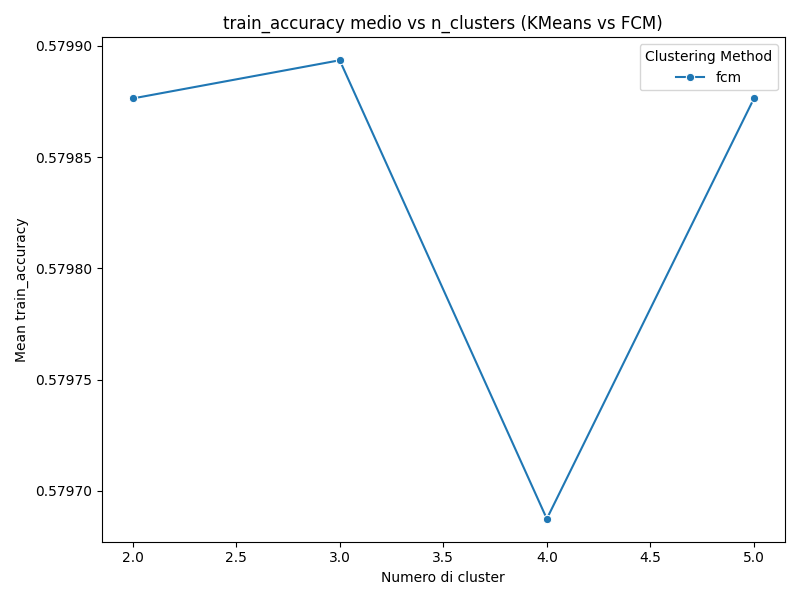
\includegraphics[width=0.8\textwidth]{../output/run_fcm/images/train/accuracy/lineplot_nclusters_train_accuracy.png}
  \caption{Lineplot - Train Accuracy - Run FCM}
  \label{fig:train_accuracy_fcm}
\end{figure}

In figura \ref{fig:train_accuracy_fcm} si può osservare come il Train Accuracy decresce intorno a 4 cluster, per poi aumentare di nuovo.

\begin{table}[H]
  \centering
  \caption{Top 5 Configurazioni per Train F1-Score - Run FCM}
  \resizebox{\textwidth}{!}{%
  \begin{tabular}{|l|c|c|c|c|c|c|c|c|c|c|}
  \hline
  \textbf{Rank} & \textbf{Normalization} & \textbf{Clusters} & \textbf{m} & \textbf{Method} & \textbf{Defuzz} & \textbf{Neighbor} & \textbf{Train F1-Score} & \textbf{Avg Max Membership} & \textbf{Avg Entropy} & \textbf{Elapsed Sec}\\
  \hline
  1 & no\_normalization & 3 & 1.2 & fcm & cog & pearson & 0.210995 & 0.446683 & 1.019679 & 43.236223 \\
  2 & no\_normalization & 2 & 1.2 & fcm & maximum & pearson & 0.210572 & 0.621032 & 0.645280 & 40.750197 \\
  3 & no\_normalization & 2 & 1.5 & fcm & maximum & pearson & 0.210572 & 0.5 & 0.693147 & 42.361609 \\
  4 & no\_normalization & 2 & 1.2 & fcm & cog & pearson & 0.210572 & 0.621032 & 0.645280 & 41.118601 \\
  5 & no\_normalization & 2 & 1.8 & fcm & maximum & pearson & 0.210572 & 0.5 & 0.693147 & 41.554277 \\
  \hline
  \end{tabular}%
  }
\end{table}

Gli F1-score sono bassi (~0.21) a causa dei valori di recall molto bassi. La configurazione con 3 cluster e cog defuzzification ottiene il miglior bilanciamento tra precision e recall.

\begin{table}[H]
  \centering
  \caption{Top 5 Configurazioni per Test RMSE - Run FCM}
  \resizebox{\textwidth}{!}{%
  \begin{tabular}{|l|c|c|c|c|c|c|c|c|c|c|}
  \hline
  \textbf{Rank} & \textbf{Normalization} & \textbf{Clusters} & \textbf{m} & \textbf{Method} & \textbf{Defuzz} & \textbf{Neighbor} & \textbf{Test RMSE} & \textbf{Avg Max Membership} & \textbf{Avg Entropy} & \textbf{Elapsed Sec}\\
  \hline
  1 & simple\_centering & 2 & 1.2 & fcm & maximum & pearson & 0.67889 & 0.5 & 0.693147 & 39.334954 \\
  2 & simple\_centering & 2 & 1.2 & fcm & cog & pearson & 0.67889 & 0.5 & 0.693147 & 39.532738 \\
  3 & simple\_centering & 2 & 1.5 & fcm & maximum & pearson & 0.67889 & 0.5 & 0.693147 & 39.051460 \\
  4 & simple\_centering & 2 & 1.5 & fcm & cog & pearson & 0.67889 & 0.5 & 0.693147 & 39.617368 \\
  5 & simple\_centering & 2 & 1.8 & fcm & maximum & pearson & 0.67889 & 0.5 & 0.693147 & 39.740233 \\
  \hline
  \end{tabular}%
  }
\end{table}

Il pattern è identico al Train RMSE: simple\_centering con 2 cluster domina. Il Test RMSE (0.6789) è leggermente migliore del Train RMSE (0.6851), suggerendo una buona generalizzazione.

\begin{table}[H]
  \centering
  \caption{Top 5 Configurazioni per Test MAE - Run FCM}
  \resizebox{\textwidth}{!}{%
  \begin{tabular}{|l|c|c|c|c|c|c|c|c|c|c|}
  \hline
  \textbf{Rank} & \textbf{Normalization} & \textbf{Clusters} & \textbf{m} & \textbf{Method} & \textbf{Defuzz} & \textbf{Neighbor} & \textbf{Test MAE} & \textbf{Avg Max Membership} & \textbf{Avg Entropy} & \textbf{Elapsed Sec}\\
  \hline
  1 & simple\_centering & 2 & 1.2 & fcm & maximum & pearson & 0.54478 & 0.5 & 0.693147 & 39.334954 \\
  2 & simple\_centering & 2 & 1.2 & fcm & cog & pearson & 0.54478 & 0.5 & 0.693147 & 39.532738 \\
  3 & simple\_centering & 2 & 1.5 & fcm & maximum & pearson & 0.54478 & 0.5 & 0.693147 & 39.051460 \\
  4 & simple\_centering & 2 & 1.5 & fcm & cog & pearson & 0.54478 & 0.5 & 0.693147 & 39.617368 \\
  5 & simple\_centering & 2 & 1.8 & fcm & maximum & pearson & 0.54478 & 0.5 & 0.693147 & 39.740233 \\
  \hline
  \end{tabular}%
  }
\end{table}

Stesso pattern del Test RMSE. Il Test MAE (0.5448) è leggermente peggiore del Train MAE (0.5107), ma la differenza è minima, indicando una buona stabilità del modello.

\begin{table}[H]
  \centering
  \caption{Top 5 Configurazioni per Test Precision - Run FCM}
  \resizebox{\textwidth}{!}{%
  \begin{tabular}{|l|c|c|c|c|c|c|c|c|c|c|}
  \hline
  \textbf{Rank} & \textbf{Normalization} & \textbf{Clusters} & \textbf{m} & \textbf{Method} & \textbf{Defuzz} & \textbf{Neighbor} & \textbf{Test Precision} & \textbf{Avg Max Membership} & \textbf{Avg Entropy} & \textbf{Elapsed Sec}\\
  \hline
  1 & zscore\_per\_user & 4 & 2.2 & fcm & maximum & pearson & 0.605029 & 0.25 & 1.386294 & 37.718682 \\
  2 & zscore\_per\_user & 4 & 2.2 & fcm & cog & pearson & 0.605029 & 0.25 & 1.386294 & 39.967926 \\
  3 & zscore\_per\_user & 4 & 2.5 & fcm & maximum & pearson & 0.605029 & 0.25 & 1.386294 & 40.161658 \\
  4 & zscore\_per\_user & 5 & 1.2 & fcm & maximum & pearson & 0.605029 & 0.2 & 1.609438 & 39.627358 \\
  5 & zscore\_per\_user & 5 & 1.5 & fcm & maximum & pearson & 0.605029 & 0.2 & 1.609438 & 50.886222 \\
  \hline
  \end{tabular}%
  }
\end{table}

A differenza del train, zscore\_per\_user domina con 4-5 cluster. I valori di Avg Max Membership sono più bassi (0.2-0.25) e Avg Entropy più alti (1.38-1.61), indicando cluster più fuzzy e sovrapposti.

\begin{figure}[H]
  \centering
  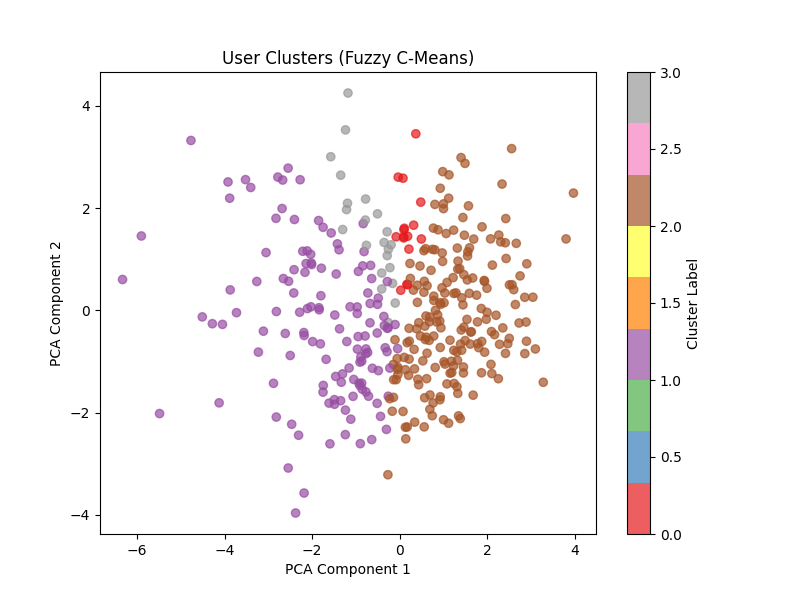
\includegraphics[width=0.8\textwidth]{../output/run_fcm/images/normalization/zscore_per_user/fuzzy_clusters/fuzzy_clusters_pca_c4_m2.2_fcm_maximum_pearson.png}
  \caption{Heatmap - Test Precision - Run FCM}
  \label{fig:test_precision_fcm}
\end{figure}

In figura \ref{fig:test_precision_fcm} riusciamo a osservare questa sfumatura dei cluster. Importante osservare come i cluster creati siano difficili da interpretare, in quanto non sono chiaramente separati.

\begin{table}[H]
  \centering
  \caption{Top 5 Configurazioni per Test Recall - Run FCM}
  \resizebox{\textwidth}{!}{%
  \begin{tabular}{|l|c|c|c|c|c|c|c|c|c|c|}
  \hline
  \textbf{Rank} & \textbf{Normalization} & \textbf{Clusters} & \textbf{m} & \textbf{Method} & \textbf{Defuzz} & \textbf{Neighbor} & \textbf{Test Recall} & \textbf{Avg Max Membership} & \textbf{Avg Entropy} & \textbf{Elapsed Sec}\\
  \hline
  1 & zscore\_per\_user & 4 & 2.2 & fcm & maximum & pearson & 0.511738 & 0.25 & 1.386294 & 37.718682 \\
  2 & zscore\_per\_user & 4 & 2.2 & fcm & cog & pearson & 0.511738 & 0.25 & 1.386294 & 39.967926 \\
  3 & zscore\_per\_user & 4 & 2.5 & fcm & maximum & pearson & 0.511738 & 0.25 & 1.386294 & 40.161658 \\
  4 & zscore\_per\_user & 5 & 1.2 & fcm & maximum & pearson & 0.511738 & 0.2 & 1.609438 & 39.627358 \\
  5 & zscore\_per\_user & 5 & 1.5 & fcm & maximum & pearson & 0.511738 & 0.2 & 1.609438 & 50.886222 \\
  \hline
  \end{tabular}%
  }
\end{table}

Il pattern è identico al Test Precision. I valori di recall (~0.51) sono molto più alti rispetto al train (~0.14), suggerendo una migliore capacità di catturare le preferenze dell'utente nel test set.

\begin{table}[H]
  \centering
  \caption{Top 5 Configurazioni per Test Accuracy - Run FCM}
  \resizebox{\textwidth}{!}{%
  \begin{tabular}{|l|c|c|c|c|c|c|c|c|c|c|}
  \hline
  \textbf{Rank} & \textbf{Normalization} & \textbf{Clusters} & \textbf{m} & \textbf{Method} & \textbf{Defuzz} & \textbf{Neighbor} & \textbf{Test Accuracy} & \textbf{Avg Max Membership} & \textbf{Avg Entropy} & \textbf{Elapsed Sec}\\
  \hline
  1 & zscore\_per\_user & 4 & 2.2 & fcm & maximum & pearson & 0.605029 & 0.25 & 1.386294 & 37.718682 \\
  2 & zscore\_per\_user & 4 & 2.2 & fcm & cog & pearson & 0.605029 & 0.25 & 1.386294 & 39.967926 \\
  3 & zscore\_per\_user & 4 & 2.5 & fcm & maximum & pearson & 0.605029 & 0.25 & 1.386294 & 40.161658 \\
  4 & zscore\_per\_user & 5 & 1.2 & fcm & maximum & pearson & 0.605029 & 0.2 & 1.609438 & 39.627358 \\
  5 & zscore\_per\_user & 5 & 1.5 & fcm & maximum & pearson & 0.605029 & 0.2 & 1.609438 & 50.886222 \\
  \hline
  \end{tabular}%
  }
\end{table}

I risultati sono identici al Test Precision, confermando che accuracy e precision coincidono anche nella fase di test. Questo pattern è consistente tra train e test.

\begin{table}[H]
  \centering
  \caption{Top 5 Configurazioni per Test F1-Score - Run FCM}
  \resizebox{\textwidth}{!}{%
  \begin{tabular}{|l|c|c|c|c|c|c|c|c|c|c|}
  \hline
  \textbf{Rank} & \textbf{Normalization} & \textbf{Clusters} & \textbf{m} & \textbf{Method} & \textbf{Defuzz} & \textbf{Neighbor} & \textbf{Test F1-Score} & \textbf{Avg Max Membership} & \textbf{Avg Entropy} & \textbf{Elapsed Sec}\\
  \hline
  1 & zscore\_per\_user & 4 & 2.2 & fcm & maximum & pearson & 0.52395 & 0.25 & 1.386294 & 37.718682 \\
  2 & zscore\_per\_user & 4 & 2.2 & fcm & cog & pearson & 0.52395 & 0.25 & 1.386294 & 39.967926 \\
  3 & zscore\_per\_user & 4 & 2.5 & fcm & maximum & pearson & 0.52395 & 0.25 & 1.386294 & 40.161658 \\
  4 & zscore\_per\_user & 5 & 1.2 & fcm & maximum & pearson & 0.52395 & 0.2 & 1.609438 & 39.627358 \\
  5 & zscore\_per\_user & 5 & 1.5 & fcm & maximum & pearson & 0.52395 & 0.2 & 1.609438 & 50.886222 \\
  \hline
  \end{tabular}%
  }
\end{table}

Gli F1-score (~0.52) sono significativamente più alti rispetto al train (~0.21) grazie ai valori di recall più elevati. Il pattern di normalizzazione e cluster è identico alle altre metriche di test.

\subsection{Conclusioni FCM}

I risultati della run FCM rivelano pattern interessanti che differiscono da quelli osservati con K-Means, evidenziando i vantaggi del clustering fuzzy nel contesto dei sistemi di raccomandazione cinematografici.

Per le metriche RMSE e MAE, FCM mostra performance simili a quelle offere da K-Means. Il Test RMSE di FCM (0.6789) è leggermente inferiore a quello di K-Means (0.6817), mentre il Test MAE di FCM (0.5448) è leggermente superiore a quello di K-Means (0.5409). Queste differenze risultano minime e dunque non sono significative.

Come per K-Means, simple\_centering domina le metriche di errore con 2 cluster, ma a differenza del clustering hard, FCM mostra valori di Avg Max Membership e Avg Entropy che variano leggermente tra le configurazioni, indicando una maggiore flessibilità nella rappresentazione delle preferenze.

Per le metriche di qualità delle raccomandazioni, FCM mostra performance identiche a K-Means, indicando che l'introduzione del clustering fuzzy non ha portato a miglioramenti significativi. In tabella \ref{tab:fcm_vs_kmeans} si può osservare un confronto tra le due tecniche.

\begin{table}[H]
  \centering
  \caption{Confronto Performance FCM vs K-Means}
  \label{tab:fcm_vs_kmeans}
  \begin{tabular}{|l|c|c|c|c|}
  \hline
  \textbf{Metrica} & \textbf{FCM Train} & \textbf{K-Means Train} & \textbf{FCM Test} & \textbf{K-Means Test} \\
  \hline
  RMSE & 0.6851 & 0.6864 & 0.6789 & 0.6817 \\
  MAE & 0.5107 & 0.5092 & 0.5448 & 0.5409 \\
  Precision & 58.9\% & 58.8\% & 60.5\% & 60.5\% \\
  Recall & 13.8\% & 13.8\% & 51.2\% & 51.2\% \\
  F1-Score & 21.1\% & 21.1\% & 52.4\% & 52.4\% \\
  \hline
  \end{tabular}
\end{table}
